\documentclass{article}
\usepackage{booktabs}
\usepackage{fontspec}
\begin{document}
\thispagestyle{empty}
\setromanfont{Times New Roman}
\begin{table}[htbp]
    %\ttfamily
    %
    \small
      \begin{tabular}{lrr}
        \toprule
      Methods  & mAP & Coverage  \\
      \midrule
      MV3D(BV+FV)  & 0.118 & 0.15 \\
      Frustum-Pointnet-v1  & 0.407 & 0.45 \\
      Frustum-Pointnet-v2  & 0.425 & 0.48 \\
      3D-VGG+RoIpool8  & 0.36  & 0.32 \\
      3D-VGG+RoIpool8(w/o maxpool)  & 0.423 & 0.41 \\
      3D-ResNet+RoIpool8  & 0.416 & 0.44 \\
      3D-ResNet+RoIpool8(Raw volume)  & 0.61  & 0.55 \\
      $A^2$-Net (APRoI8)  & 0.711 & 0.67 \\
      $A^2$-Net w/o Neighbor Loss  & 0.865 & 0.72 \\
      $A^2$-Net  & 0.891 & 0.91 \\
      \bottomrule
      \end{tabular}%
      %\caption{The results of detection and threading comparing with other 3D object detection methods.}
    \end{table}%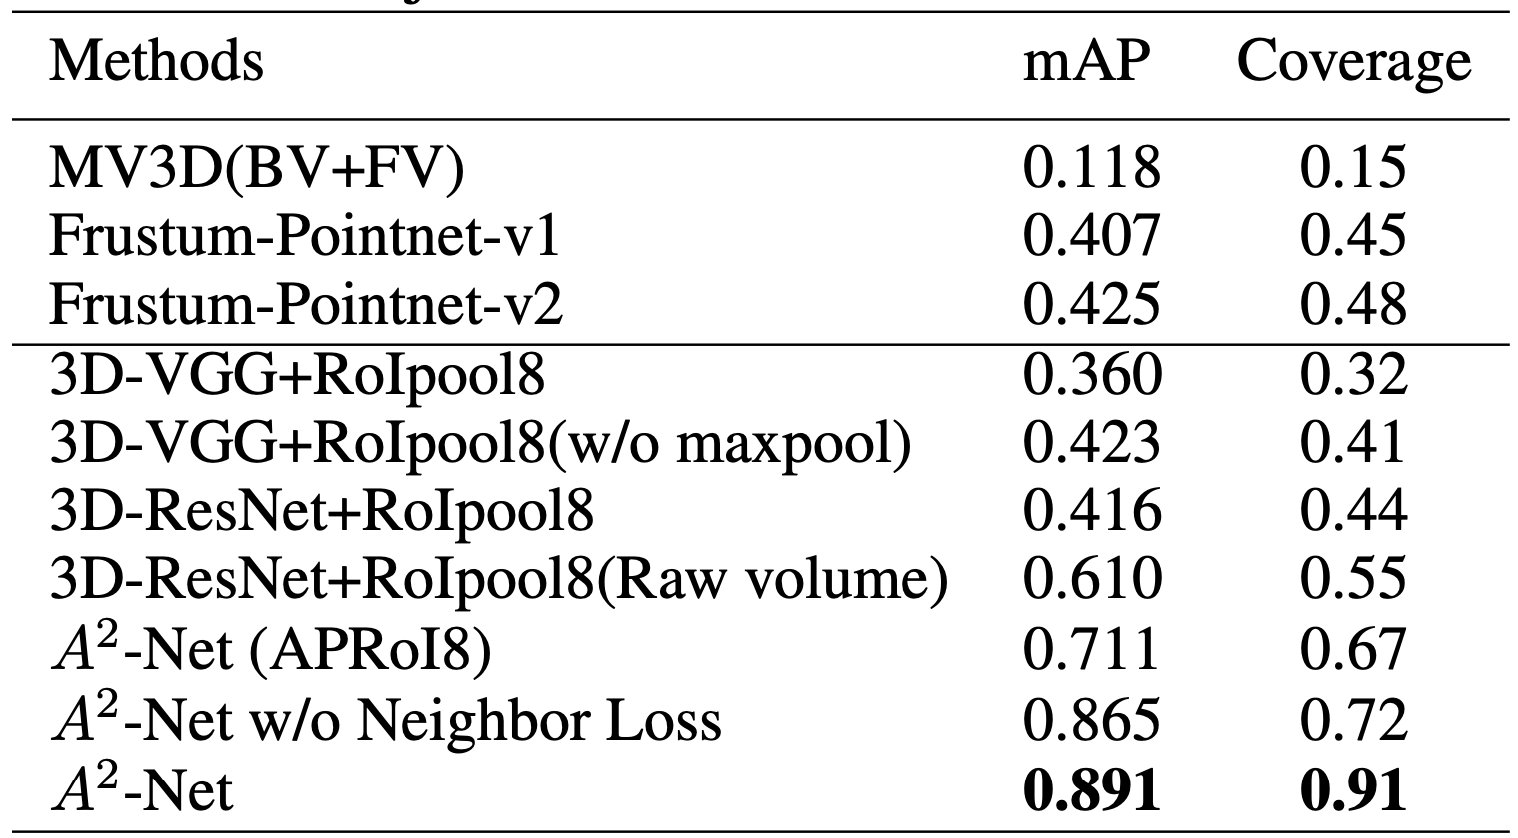
\includegraphics[width=0.45\columnwidth]{detection.png}}
\end{document}